\documentclass[a4paper]{article}
\usepackage[a4paper,margin=0mm]{geometry}
\usepackage{fontspec}
\usepackage{unicode-math}
\usepackage{tikz}
\usepackage[table]{xcolor}
\usepackage[absolute]{textpos}
\usepackage{array}
\usepackage{multirow}

\setmainfont{Libertinus Serif}
\setsansfont{Libertinus Sans}
\setmathfont{Libertinus Math}

\definecolor{accent}{HTML}{0F6A52}
\definecolor{badge}{HTML}{A9CFC2}
\definecolor{ink}{HTML}{2A2E30}

\setlength{\TPHorizModule}{1mm}
\setlength{\TPVertModule}{1mm}
\setlength{\parindent}{0pt}
\setlength{\parskip}{0pt}
\emergencystretch=3em
\abovedisplayskip=4pt plus 2pt minus 2pt \belowdisplayskip=4pt plus 2pt minus 2pt \abovedisplayshortskip=2pt \belowdisplayshortskip=2pt
\pagestyle{empty}

\newcommand{\LCOL}{16mm}
\newcommand{\RCOL}{111mm}
\newcommand{\COLW}{83mm}

\newcommand{\topicheader}[2]{%
\begin{textblock*}{194mm}(16mm,10mm)
\begin{tikzpicture}
\node[fill=accent,text=white,font=\sffamily\bfseries\fontsize{13}{13}\selectfont,
      minimum width=9mm,minimum height=9mm,inner sep=0pt] at (4.5mm,-4.5mm) {#1};
\node[font=\sffamily\bfseries\fontsize{15}{16}\selectfont,text=ink,anchor=west] at (12mm,-4.5mm) {#2};
\end{tikzpicture}
\end{textblock*}
\begin{textblock*}{194mm}(16mm,22.5mm)

\begin{tikzpicture}
\fill[accent] (0,0) rectangle (194mm,0.5mm);
\end{tikzpicture}
\end{textblock*}
}

\newcommand{\pagefooter}[1]{%
\begin{textblock*}{194mm}(8mm,286.41mm)
  
\begin{tikzpicture}
    \fill[accent] (0,0) rectangle (194mm,0.6mm);
  \end{tikzpicture}
\end{textblock*}
\begin{textblock*}{63.59mm}(8mm,288.27mm)
  {\sffamily\bfseries\color{accent}\fontsize{13}{16}\selectfont SAT 1200+}
\end{textblock*}
\begin{textblock*}{10mm}(188mm,288.27mm)
  \centering{\sffamily\color{accent}\fontsize{14}{16}\selectfont #1}
\end{textblock*}
}

\newcommand{\colrule}[2]{%
\begin{textblock*}{1mm}(105mm,#1mm)
\begin{tikzpicture}
\draw[black!65,line width=0.5pt] (0,0) -- (0,#2mm);
\end{tikzpicture}
\end{textblock*}
}

\newcommand{\setkicker}[2]{%
{\sffamily\bfseries\fontsize{12}{14}\selectfont #1.}\ {\itshape\fontsize{11}{14}\selectfont\color{black!75} #2}\par\vspace{2mm}%
}

\setlength{\fboxsep}{1.4pt}
\setlength{\fboxrule}{0.5pt}
\newcommand{\pnum}[1]{\fcolorbox{ink}{white}{\sffamily\bfseries\fontsize{8}{8}\selectfont #1}~}

% ---- SAT-style multiple-choice block (2x2 grid of short choices) ----
\newcommand{\satq}[6]{%
\noindent\pnum{#1} #2\par\nobreak\vspace{2mm}%
\noindent\hspace*{7mm}\begin{tabular}[t]{@{}p{32mm}p{32mm}@{}}
(A) #3 & (B) #4 \\[2mm]
(C) #5 & (D) #6 \\
\end{tabular}\par\vspace{5.5mm}%
}

% ---- stacked choices for long ones ----
\newcommand{\satqw}[6]{%
\noindent\pnum{#1} #2\par\nobreak\vspace{2mm}%
\noindent\hspace*{7mm}(A) #3\par\vspace{1.6mm}%
\noindent\hspace*{7mm}(B) #4\par\vspace{1.6mm}%
\noindent\hspace*{7mm}(C) #5\par\vspace{1.6mm}%
\noindent\hspace*{7mm}(D) #6\par\vspace{5.5mm}%
}

% ---- student-produced response (grid-in) ----
\newcommand{\satg}[2]{%
\noindent\pnum{#1} {\sffamily\bfseries\fontsize{7}{8}\selectfont\color{accent}GRID-IN}\ #2\par\nobreak\vspace{2.5mm}%
\noindent\hspace*{7mm}{\sffamily\fontsize{8.5}{10}\selectfont Answer:}\ \rule[-1.2mm]{28mm}{0.4pt}\par\vspace{5.5mm}%
}

% ---- worked-solution entry ----
\newcommand{\solitem}[4]{%
\noindent\pnum{#1} {\bfseries #2}\ —\ #3\ {\itshape\color{accent}[#4]}\par\vspace{2.1mm}%
}

\usetikzlibrary{arrows.meta}
\newsavebox{\figsave}
\newcommand{\figbox}[1]{\par\vspace{1.8mm}\sbox{\figsave}{#1}\noindent\hfill\ifdim\wd\figsave>\hsize\resizebox{\hsize}{!}{\usebox{\figsave}}\else\usebox{\figsave}\fi\hfill\null\par\vspace{0.8mm}}
\arrayrulecolor{accent}
\setlength{\arrayrulewidth}{0.7pt}
\renewcommand{\arraystretch}{1.3}

\usepackage{multicol}
\usepackage{fancyhdr}
\usepackage{needspace}
\newcommand{\pgoff}{0}
\renewcommand{\solitem}[4]{\noindent\parbox[t]{\linewidth}{\raggedright\pnum{#1} {\bfseries #2}\ ---\ #3\ {\itshape\color{accent}[#4]}}\par\vspace{3.6mm}}
\newcommand{\solkicker}[2]{\Needspace{38mm}\vspace{1.5mm}{\sffamily\bfseries\fontsize{12.5}{15}\selectfont #1.}\ {\itshape\fontsize{11}{14}\selectfont\color{black!75} #2}\par\vspace{3mm}}
\renewcommand{\satqw}[6]{%
\noindent\pnum{#1} #2\par\nobreak\vspace{2mm}%
\noindent\hangindent=13mm\hangafter=1\hspace*{7mm}(A)~#3\par\vspace{1.6mm}%
\noindent\hangindent=13mm\hangafter=1\hspace*{7mm}(B)~#4\par\vspace{1.6mm}%
\noindent\hangindent=13mm\hangafter=1\hspace*{7mm}(C)~#5\par\vspace{1.6mm}%
\noindent\hangindent=13mm\hangafter=1\hspace*{7mm}(D)~#6\par\vspace{5.5mm}%
}
\newcommand{\solkitem}[5]{\noindent\parbox[t]{\linewidth}{\vspace{1.5mm}{\sffamily\bfseries\fontsize{12.5}{15}\selectfont #1.}\ {\itshape\fontsize{11}{14}\selectfont\color{black!75} Worked solutions}\par\vspace{3mm}\raggedright\pnum{#2} {\bfseries #3}\ ---\ #4\ {\itshape\color{accent}[#5]}}\par\vspace{3.6mm}}
\fancypagestyle{solstyle}{\fancyhf{}\renewcommand{\headrulewidth}{0pt}\renewcommand{\footrulewidth}{0pt}%
 \fancyhead[L]{\topicheader{8}{Hard Circles, Area \& Volume}}%
 \fancyfoot[L]{\pagefooter{\the\numexpr\value{page}+\pgoff\relax}}}

\begin{document}
\topicheader{8}{Hard Circles, Area \& Volume}
\pagefooter{1}
\colrule{32}{238}
\mbox{}%
\begin{textblock*}{\COLW}(\LCOL,32mm)
{\fontsize{10}{12.5}\selectfont
\setkicker{Set 1}{Bridge: the core moves, one problem each.}
\satq{1}{The graph of $(x-2)^2+(y+5)^2=36$ in the $xy$-plane is a circle. What is the length of a diameter of the circle?}{$6$}{$12$}{$36$}{$72$}
\satq{2}{A circle in the $xy$-plane has center $(1,-2)$ and radius $5$. Which of the following points lies \emph{inside} the circle?}{$(3,0)$}{$(-3,-5)$}{$(1,3)$}{$(6,1)$}
\satg{3}{A circle has radius $9$. An arc of the circle has a central angle of $80^\circ$, and the length of the arc is $k\pi$. What is the value of $k$?}
\satq{4}{A circle has a diameter of $24$. A sector of this circle has an area of $60\pi$. What is the measure, in degrees, of the central angle of the sector?}{$37.5$}{$60$}{$75$}{$150$}
\satq{5}{Points $A$ and $B$ lie on a circle with center $O$, and $\angle AOB=100^\circ$. Point $C$ lies on the \emph{major} arc $AB$ (the longer arc). What is the measure, in degrees, of $\angle ACB$?}{$50^\circ$}{$100^\circ$}{$130^\circ$}{$200^\circ$}
\satq{6}{A sphere has a volume of $288\pi$ cubic centimeters. What is the surface area, in square centimeters, of the sphere?}{$36 \pi$}{$72 \pi$}{$144 \pi$}{$576 \pi$}
\satq{7}{A tank shaped like a rectangular box is $2$ m long, $1.5$ m wide and $0.8$ m deep. How many liters of water does it hold when full? ($1$ cubic meter $=1000$ liters)}{$2.4$}{$240$}{$2{,}400$}{$24{,}000$}
}
\end{textblock*}
\begin{textblock*}{\COLW}(\RCOL,32mm)
{\fontsize{10}{12.5}\selectfont
\setkicker{Set 1 (cont.)}{Bridge}
\satq{8}{Two right circular cones are similar. The height of the larger cone is $3$ times the height of the smaller cone, and the smaller cone has a volume of $40$ cubic centimeters. What is the volume, in cubic centimeters, of the larger cone?}{$3{,}240$}{$1{,}080$}{$360$}{$120$}
\satg{9}{An arc of length $2\pi$ lies on a circle of radius $6$. What is the measure, in degrees, of the central angle that intercepts the arc?}
\satq{10}{A region is made of a $10$-by-$6$ rectangle together with a semicircle whose diameter is a $6$-unit side of the rectangle (the semicircle lies outside the rectangle). What is the area of the region?}{$60 + 36 \pi$}{$60 + 18 \pi$}{$60 + 9 \pi$}{$60 + \frac{9 \pi}{2}$}
\satq{11}{Water is pumped into an empty cylindrical tank with a base radius of $4$ feet at a constant rate of $24\pi$ cubic feet per minute. By how many feet does the water level rise each minute?}{$0.375$}{$1.5$}{$3$}{$6$}
\satg{12}{The equation $x^2+y^2-6x+10y+18=0$ defines a circle in the $xy$-plane. What is the radius of the circle?}
\vspace{3mm}
\setkicker{Set 2}{Circles in the plane: equations, tangents, chords, angles, arcs.}
\satq{1}{In the $xy$-plane, the graph of $x^2+y^2+8x-2y+k=0$ is a circle with radius $5$. What is the value of $k$?}{$-8$}{$8$}{$12$}{$42$}
\satg{2}{The graph of $x^2+y^2-4x+6y-12=0$ is a circle in the $xy$-plane that crosses the $x$-axis at two points. What is the distance between these two points?}
}
\end{textblock*}
\clearpage
\topicheader{8}{Hard Circles, Area \& Volume}
\pagefooter{2}
\colrule{32}{238}
\mbox{}%
\begin{textblock*}{\COLW}(\LCOL,32mm)
{\fontsize{10}{12.5}\selectfont
\setkicker{Set 2 (cont.)}{Circles in the plane}
\satq{3}{In the $xy$-plane, a circle has center $(2,-1)$. A line is tangent to the circle at the point $(5,3)$. Which of the following points also lies on this line?}{$(9,6)$}{$(8,7)$}{$(9,0)$}{$(8,-1)$}
\satq{4}{In the $xy$-plane, the circle $x^2+y^2=k$ is tangent to the line $3x-4y=40$. What is the value of $k$?}{$64$}{$8$}{$40$}{$1{,}600$}
\satg{5}{A circle has radius $17$. Chord $AB$ has length $30$ and $M$ is the midpoint of $AB$. The line through the center $O$ and $M$ meets the circle again at point $N$ on the short arc $AB$ (see the figure). What is the length of $\overline{MN}$?\figbox{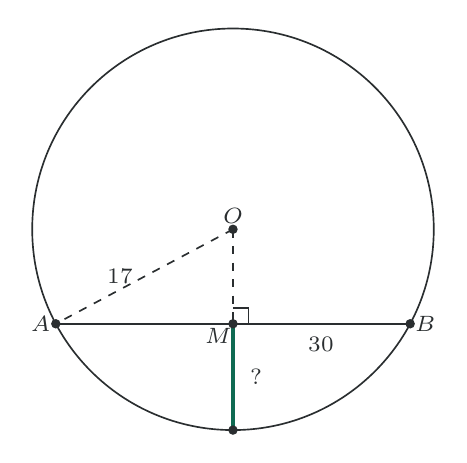
\begin{tikzpicture}[line width=0.6pt,ink,every node/.style={font=\footnotesize}]
\draw (0.000mm,0.000mm) circle (25.500mm);
\draw (-22.500mm,-12.000mm) -- (22.500mm,-12.000mm);
\draw[dashed] (0.000mm,0.000mm) -- (0.000mm,-12.000mm);
\draw[dashed] (0.000mm,0.000mm) -- (-22.500mm,-12.000mm);
\draw[accent,line width=1.4pt] (0.000mm,-12.000mm) -- (0.000mm,-25.500mm);
\draw[ink,line width=0.4pt] (0.000mm,-10.000mm) -- (2.000mm,-10.000mm) -- (2.000mm,-12.000mm);
\fill[ink] (0.000mm,0.000mm) circle (0.6mm); \node[above,inner sep=1.5pt] at (0.000mm,0.000mm) {$O$};
\fill[ink] (-22.500mm,-12.000mm) circle (0.6mm); \node[left,inner sep=1.5pt] at (-22.500mm,-12.000mm) {$A$};
\fill[ink] (22.500mm,-12.000mm) circle (0.6mm); \node[right,inner sep=1.5pt] at (22.500mm,-12.000mm) {$B$};
\fill[ink] (0.000mm,-12.000mm) circle (0.6mm); \node[below left,inner sep=1.5pt,xshift=0.5pt] at (0.000mm,-12.000mm) {$M$};
\fill[ink] (0.000mm,-25.500mm) circle (0.6mm);
\node[below=1pt] at (11.250mm,-12.000mm) {$30$};
\node[left=0.5pt] at (-11.250mm,-6.000mm) {$17$};
\node[right=1pt] at (0.600mm,-18.750mm) {$?$};
\end{tikzpicture}}}
\satq{6}{In the figure, $\overline{AB}$ is a diameter of the circle with center $O$, point $C$ lies on the circle, and $\angle BAC=28^\circ$. What is the measure, in degrees, of the minor arc $AC$?\figbox{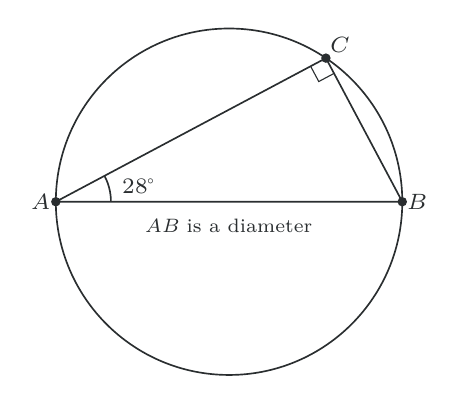
\begin{tikzpicture}[line width=0.6pt,ink,every node/.style={font=\footnotesize}]
\draw (0.000mm,0.000mm) circle (22.000mm);
\draw (-22.000mm,0.000mm) -- (22.000mm,0.000mm) -- (12.302mm,18.239mm) -- cycle;
\draw[ink,line width=0.4pt] (10.360mm,17.206mm) -- (11.393mm,15.264mm) -- (13.335mm,16.296mm);
\draw (-15.000mm,0.000mm) arc[start angle=0,end angle=28.000,radius=7mm];
\node[right] at (-14.800mm,1.900mm) {$28^\circ$};
\fill[ink] (-22.000mm,0.000mm) circle (0.6mm); \node[left,inner sep=1.5pt] at (-22.000mm,0.000mm) {$A$};
\fill[ink] (22.000mm,0.000mm) circle (0.6mm); \node[right,inner sep=1.5pt] at (22.000mm,0.000mm) {$B$};
\fill[ink] (12.302mm,18.239mm) circle (0.6mm); \node[above right,inner sep=1.5pt] at (12.302mm,18.239mm) {$C$};
\node[below=1pt] at (0.000mm,-0.500mm) {\scriptsize $AB$ is a diameter};
\end{tikzpicture}}}{$152$}{$124$}{$62$}{$56$}
}
\end{textblock*}
\begin{textblock*}{\COLW}(\RCOL,32mm)
{\fontsize{10}{12.5}\selectfont
\setkicker{Set 2 (cont.)}{Circles in the plane}
\satq{7}{From a point $E$ outside a circle with center $O$, tangent segments $\overline{EA}$ and $\overline{EU}$ are drawn to the circle, touching it at $A$ and $U$, with $\angle AEU=50^\circ$. Point $C$ lies on the major arc $AU$. What is the measure, in degrees, of $\angle ACU$?}{$130^\circ$}{$115^\circ$}{$65^\circ$}{$50^\circ$}
\satg{8}{A circle has center $O$ and radius $6$. From a point $E$ outside the circle, tangent segments $\overline{EA}$ and $\overline{EU}$ of length $8$ are drawn (see the figure). Segment $\overline{OE}$ crosses the circle at $P$. What is the length of $\overline{PE}$?\figbox{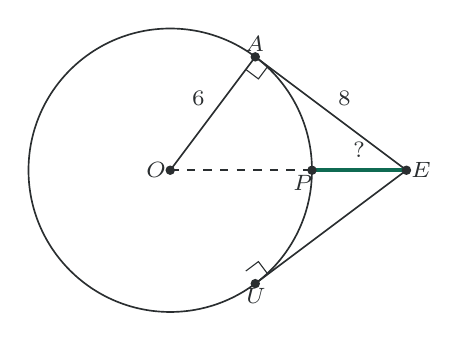
\begin{tikzpicture}[line width=0.6pt,ink,every node/.style={font=\footnotesize}]
\draw (0.000mm,0.000mm) circle (18.000mm);
\draw (0.000mm,0.000mm) -- (10.800mm,14.400mm) -- (30.000mm,0.000mm) -- (10.800mm,-14.400mm);
\draw[dashed] (0.000mm,0.000mm) -- (30.000mm,0.000mm);
\draw[accent,line width=1.4pt] (18.000mm,0.000mm) -- (30.000mm,0.000mm);
\draw[ink,line width=0.4pt] (9.600mm,12.800mm) -- (11.200mm,11.600mm) -- (12.400mm,13.200mm);
\draw[ink,line width=0.4pt] (9.600mm,-12.800mm) -- (11.200mm,-11.600mm) -- (12.400mm,-13.200mm);
\fill[ink] (0.000mm,0.000mm) circle (0.6mm); \node[left,inner sep=1.5pt] at (0.000mm,0.000mm) {$O$};
\fill[ink] (10.800mm,14.400mm) circle (0.6mm); \node[above,inner sep=1.5pt] at (10.800mm,14.400mm) {$A$};
\fill[ink] (10.800mm,-14.400mm) circle (0.6mm); \node[below,inner sep=1.5pt] at (10.800mm,-14.400mm) {$U$};
\fill[ink] (30.000mm,0.000mm) circle (0.6mm); \node[right,inner sep=1.5pt] at (30.000mm,0.000mm) {$E$};
\fill[ink] (18.000mm,0.000mm) circle (0.6mm); \node[below left,inner sep=1.5pt,xshift=1pt] at (18.000mm,0.000mm) {$P$};
\node[above left=-1pt] at (5.400mm,7.200mm) {$6$};
\node[above right=-1pt] at (20.400mm,7.200mm) {$8$};
\node[above=1pt] at (24.000mm,0.000mm) {$?$};
\end{tikzpicture}}}
\satq{9}{A sector of a circle has a central angle of $60^\circ$ and an area of $24\pi$. What is the length of the arc of the sector?}{$4 \pi$}{$2 \pi$}{$12 \pi$}{$24 \pi$}
\satq{10}{A sector of a circle has radius $9$ and a central angle of $\frac{5\pi}{6}$ radians. What is the area of the sector?}{$\frac{15 \pi}{4}$}{$\frac{15 \pi}{2}$}{$\frac{135 \pi}{2}$}{$\frac{135 \pi}{4}$}
}
\end{textblock*}
\clearpage
\topicheader{8}{Hard Circles, Area \& Volume}
\pagefooter{3}
\colrule{32}{238}
\mbox{}%
\begin{textblock*}{\COLW}(\LCOL,32mm)
{\fontsize{10}{12.5}\selectfont
\setkicker{Set 2 (cont.)}{Circles in the plane}
\satq{11}{A right triangle has legs of length $9$ and $12$. A circle is inscribed in the triangle, touching all three sides. What is the area of the part of the triangle that lies outside the circle?\figbox{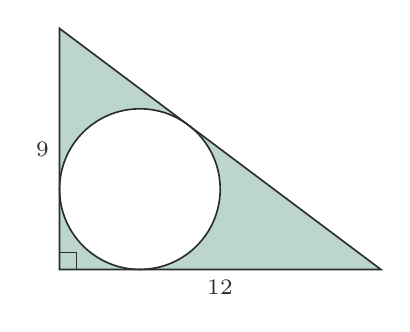
\begin{tikzpicture}[line width=0.6pt,ink,every node/.style={font=\footnotesize}]
\fill[accent!28] (0.000mm,0.000mm) -- (40.800mm,0.000mm) -- (0.000mm,30.600mm) -- cycle;
\filldraw[fill=white] (10.200mm,10.200mm) circle (10.200mm);
\draw (0.000mm,0.000mm) -- (40.800mm,0.000mm) -- (0.000mm,30.600mm) -- cycle;
\draw[ink,line width=0.4pt] (2.200mm,0.000mm) -- (2.200mm,2.200mm) -- (0.000mm,2.200mm);
\node[left] at (0.000mm,15.300mm) {$9$};
\node[below] at (20.400mm,0.000mm) {$12$};
\end{tikzpicture}}}{$54 - 36 \pi$}{$54 - 9 \pi$}{$54 - 6 \pi$}{$54 - 3 \pi$}
\satq{12}{A circle in the $xy$-plane has center $(-4,6)$ and is tangent to the line $y=-2$. An equation of the circle is $(x+4)^2+(y-6)^2=k$. What is the value of $k$?}{$8$}{$16$}{$36$}{$64$}
\satg{13}{Segment $\overline{PQ}$ with endpoints $P(1,2)$ and $Q(9,8)$ is a diameter of a circle in the $xy$-plane. The circle has equation $x^2+y^2+ax+by+c=0$, where $a$, $b$ and $c$ are constants. What is the value of $a+b+c$?}
\satq{14}{In the $xy$-plane, the line $y=x+k$ is tangent to the circle $x^2+y^2=18$. Which of the following could be the value of $k$?}{$3 \sqrt{2}$}{$9$}{$18$}{$6$}
}
\end{textblock*}
\begin{textblock*}{\COLW}(\RCOL,32mm)
{\fontsize{10}{12.5}\selectfont
\setkicker{Set 3}{Areas: shaded regions, composite figures and scaling.}
\satq{1}{Two circles share the same center. A chord of the larger circle is tangent to the smaller circle and has length $24$ (see the figure). What is the area of the region between the two circles?\figbox{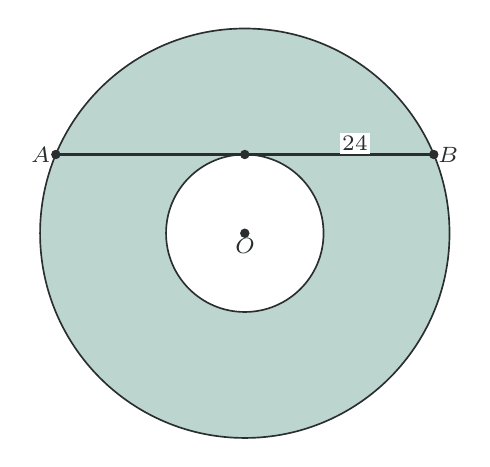
\begin{tikzpicture}[line width=0.6pt,ink,every node/.style={font=\footnotesize}]
\fill[accent!28,even odd rule] (0.000mm,0.000mm) circle (26.000mm) (0.000mm,0.000mm) circle (10.000mm);
\draw (0.000mm,0.000mm) circle (26.000mm); \draw (0.000mm,0.000mm) circle (10.000mm);
\draw[line width=0.9pt] (-24.000mm,10.000mm) -- (24.000mm,10.000mm);
\fill[ink] (0.000mm,0.000mm) circle (0.6mm); \node[below,inner sep=1.5pt] at (0.000mm,0.000mm) {$O$};
\fill[ink] (-24.000mm,10.000mm) circle (0.6mm); \node[left,inner sep=1.5pt] at (-24.000mm,10.000mm) {$A$};
\fill[ink] (24.000mm,10.000mm) circle (0.6mm); \node[right,inner sep=1.5pt] at (24.000mm,10.000mm) {$B$};
\fill[ink] (0.000mm,10.000mm) circle (0.6mm);
\node[above,fill=white,inner sep=1pt] at (14.000mm,10.000mm) {$24$};
\end{tikzpicture}}}{$12 \pi$}{$288 \pi$}{$576 \pi$}{$144 \pi$}
\satq{2}{Four congruent circles lie inside a square of side $20$. Each circle touches the two nearest sides of the square and the two neighboring circles (see the figure). What is the area of the part of the square outside all four circles?\figbox{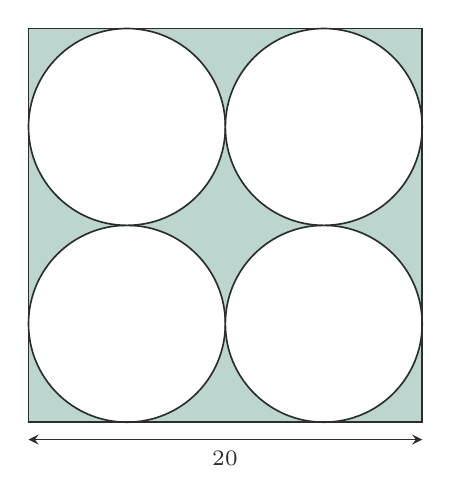
\begin{tikzpicture}[line width=0.6pt,ink,every node/.style={font=\footnotesize}]
\fill[accent!28] (0.000mm,0.000mm) rectangle (50.000mm,50.000mm);
\filldraw[fill=white] (12.500mm,12.500mm) circle (12.500mm);
\filldraw[fill=white] (12.500mm,37.500mm) circle (12.500mm);
\filldraw[fill=white] (37.500mm,12.500mm) circle (12.500mm);
\filldraw[fill=white] (37.500mm,37.500mm) circle (12.500mm);
\draw (0.000mm,0.000mm) rectangle (50.000mm,50.000mm);
\draw[<->,>=stealth] (0.000mm,-2.200mm) -- (50.000mm,-2.200mm) node[midway,below=0.5pt] {$20$};
\end{tikzpicture}}}{$400 - 25 \pi$}{$400 - 40 \pi$}{$400 - 100 \pi$}{$400 - 400 \pi$}
}
\end{textblock*}
\clearpage
\topicheader{8}{Hard Circles, Area \& Volume}
\pagefooter{4}
\colrule{32}{238}
\mbox{}%
\begin{textblock*}{\COLW}(\LCOL,32mm)
{\fontsize{10}{12.5}\selectfont
\setkicker{Set 3 (cont.)}{Areas and scaling}
\satq{3}{The figure shows a region made of a rectangle and two semicircles, one on each of the two short sides of the rectangle. The long side of the rectangle is $3$ times the short side. The perimeter of the whole region is $48+8\pi$. What is the area of the region?\figbox{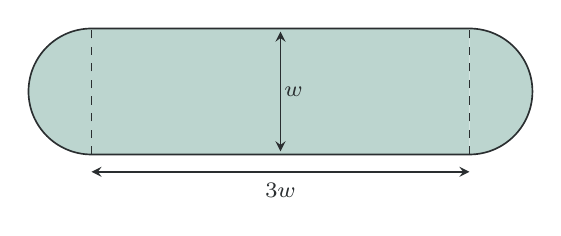
\begin{tikzpicture}[line width=0.6pt,ink,every node/.style={font=\footnotesize}]
\fill[accent!28] (0.000mm,0.000mm) rectangle (48.000mm,16.000mm);
\fill[accent!28] (48.000mm,0.000mm) arc[start angle=-90,end angle=90,radius=8.000mm] -- cycle;
\fill[accent!28] (0.000mm,0.000mm) arc[start angle=270,end angle=90,radius=8.000mm] -- cycle;
\draw (0.000mm,0.000mm) -- (48.000mm,0.000mm) arc[start angle=-90,end angle=90,radius=8.000mm] -- (0.000mm,16.000mm) arc[start angle=90,end angle=270,radius=8.000mm] -- cycle;
\draw[dashed] (0.000mm,0.000mm) -- (0.000mm,16.000mm); \draw[dashed] (48.000mm,0.000mm) -- (48.000mm,16.000mm);
\draw[<->,>=stealth] (24.000mm,0.400mm) -- (24.000mm,15.600mm) node[midway,right,inner sep=1pt] {$w$};
\draw[<->,>=stealth] (0.000mm,-2.200mm) -- (48.000mm,-2.200mm) node[midway,below=0.5pt] {$3w$};
\end{tikzpicture}}}{$192 + 8 \pi$}{$192 + 16 \pi$}{$192 + 32 \pi$}{$192 + 64 \pi$}
\satg{4}{Square $ABCD$ has side length $12$. One arc of radius $12$ is centered at $A$ and passes through $B$ and $D$. A second arc of radius $12$ is centered at $C$ and also passes through $B$ and $D$ (see the figure). The area of the shaded region where the two arcs overlap is $a\pi-b$. What is the value of $a+b$?\figbox{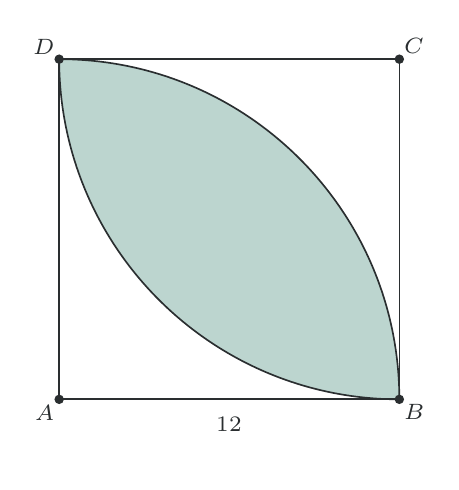
\begin{tikzpicture}[line width=0.6pt,ink,every node/.style={font=\footnotesize}]
\path[use as bounding box] (-4.000mm,-8.000mm) rectangle (47.200mm,47.200mm);
\begin{scope}\clip (0.000mm,0.000mm) circle (43.200mm); \fill[accent!28] (43.200mm,43.200mm) circle (43.200mm);\end{scope}
\draw (0.000mm,0.000mm) rectangle (43.200mm,43.200mm);
\draw (43.200mm,0.000mm) arc[start angle=0,end angle=90,radius=43.200mm];
\draw (0.000mm,43.200mm) arc[start angle=180,end angle=270,radius=43.200mm];
\fill[ink] (0.000mm,0.000mm) circle (0.6mm); \node[below left,inner sep=1.5pt] at (0.000mm,0.000mm) {$A$};
\fill[ink] (43.200mm,0.000mm) circle (0.6mm); \node[below right,inner sep=1.5pt] at (43.200mm,0.000mm) {$B$};
\fill[ink] (43.200mm,43.200mm) circle (0.6mm); \node[above right,inner sep=1.5pt] at (43.200mm,43.200mm) {$C$};
\fill[ink] (0.000mm,43.200mm) circle (0.6mm); \node[above left,inner sep=1.5pt] at (0.000mm,43.200mm) {$D$};
\node[below=1pt] at (21.600mm,-0.600mm) {$12$};
\end{tikzpicture}}}
\satq{5}{A square with side length $10$ is inscribed in a circle (all four vertices lie on the circle). What is the area of the region inside the circle but outside the square?}{$50 \pi - 100$}{$50 \pi$}{$100 \pi - 100$}{$200 \pi - 100$}
}
\end{textblock*}
\begin{textblock*}{\COLW}(\RCOL,32mm)
{\fontsize{10}{12.5}\selectfont
\setkicker{Set 3 (cont.)}{Areas and scaling}
\satq{6}{Two circles have the same center. The radius of the larger circle is $25\%$ greater than the radius of the smaller circle. The region between the circles is what percent of the area of the larger circle?}{$25\%$}{$56.25\%$}{$64\%$}{$36\%$}
\satq{7}{In the figure, $O$ is the center of a circle of radius $6$ and $\angle AOB=60^\circ$. What is the area of the shaded region bounded by chord $\overline{AB}$ and the minor arc $AB$?\figbox{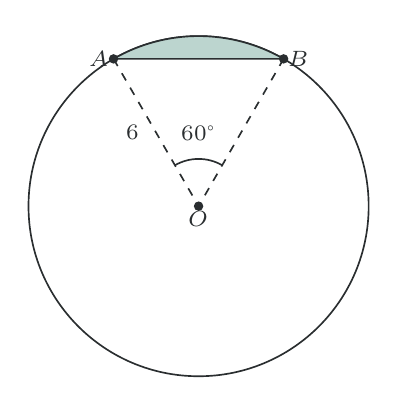
\begin{tikzpicture}[line width=0.6pt,ink,every node/.style={font=\footnotesize}]
\draw (0.000mm,0.000mm) circle (21.600mm);
\fill[accent!28] (10.800mm,18.706mm) arc[start angle=60.000,end angle=120.000,radius=21.600mm] -- cycle;
\draw (10.800mm,18.706mm) arc[start angle=60.000,end angle=120.000,radius=21.600mm] -- cycle;
\draw[dashed] (-10.800mm,18.706mm) -- (0.000mm,0.000mm) -- (10.800mm,18.706mm);
\draw (3.000mm,5.196mm) arc[start angle=60.000,end angle=120.000,radius=6mm];
\node at (0.000mm,9.200mm) {$60^\circ$};
\fill[ink] (0.000mm,0.000mm) circle (0.6mm); \node[below,inner sep=1.5pt] at (0.000mm,0.000mm) {$O$};
\fill[ink] (-10.800mm,18.706mm) circle (0.6mm); \node[left,inner sep=1.5pt] at (-10.800mm,18.706mm) {$A$};
\fill[ink] (10.800mm,18.706mm) circle (0.6mm); \node[right,inner sep=1.5pt] at (10.800mm,18.706mm) {$B$};
\node[left=1pt] at (-5.900mm,9.353mm) {$6$};
\end{tikzpicture}}}{$6 \pi$}{$6 \pi - 9$}{$6 \pi - 9 \sqrt{3}$}{$6 \pi - 18 \sqrt{3}$}
\satg{8}{The radius of a circle is increased by $p\%$, and as a result the area of the circle increases by $69\%$. What is the value of $p$?}
\satq{9}{An equilateral triangle with side length $6$ is inscribed in a circle (all three vertices lie on the circle). What is the area of the circle?}{$36 \pi$}{$12 \pi$}{$9 \pi$}{$3 \pi$}
}
\end{textblock*}
\clearpage
\topicheader{8}{Hard Circles, Area \& Volume}
\pagefooter{5}
\colrule{32}{238}
\mbox{}%
\begin{textblock*}{\COLW}(\LCOL,32mm)
{\fontsize{10}{12.5}\selectfont
\setkicker{Set 3 (cont.)}{Areas and scaling}
\satq{10}{Two circles with radii $4$ and $9$ are externally tangent. A line is tangent to the smaller circle at $P$ and to the larger circle at $Q$, and both circles lie on the same side of the line (see the figure). What is the length of $\overline{PQ}$?\figbox{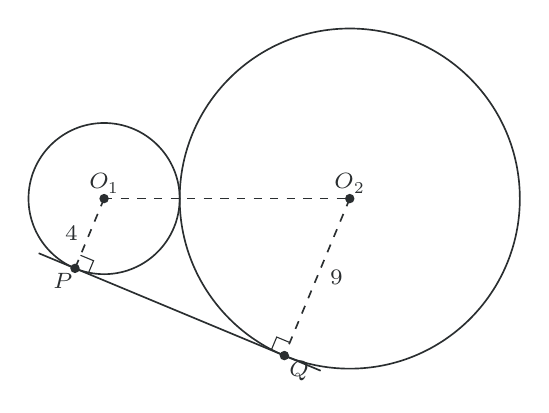
\begin{tikzpicture}[line width=0.6pt,ink,every node/.style={font=\footnotesize}]
\draw (0.000mm,0.000mm) circle (9.600mm); \draw (31.200mm,0.000mm) circle (21.600mm);
\draw (-8.308mm,-6.938mm) -- (27.508mm,-21.862mm);
\draw[dashed] (0.000mm,0.000mm) -- (-3.692mm,-8.862mm); \draw[dashed] (31.200mm,0.000mm) -- (22.892mm,-19.938mm);
\draw[dashed] (0.000mm,0.000mm) -- (31.200mm,0.000mm);
\draw[ink,line width=0.4pt] (-3.000mm,-7.200mm) -- (-1.338mm,-7.892mm) -- (-2.031mm,-9.554mm);
\draw[ink,line width=0.4pt] (23.585mm,-18.277mm) -- (21.923mm,-17.585mm) -- (21.231mm,-19.246mm);
\fill[ink] (0.000mm,0.000mm) circle (0.6mm); \node[above,inner sep=1.5pt] at (0.000mm,0.000mm) {$O_1$};
\fill[ink] (31.200mm,0.000mm) circle (0.6mm); \node[above,inner sep=1.5pt] at (31.200mm,0.000mm) {$O_2$};
\fill[ink] (-3.692mm,-8.862mm) circle (0.6mm); \node[below left,inner sep=1.5pt] at (-3.692mm,-8.862mm) {$P$};
\fill[ink] (22.892mm,-19.938mm) circle (0.6mm); \node[below right,inner sep=1.5pt] at (22.892mm,-19.938mm) {$Q$};
\node[left=0.5pt] at (-1.846mm,-4.431mm) {$4$};
\node[right=0.5pt] at (27.346mm,-9.969mm) {$9$};
\end{tikzpicture}}}{$5$}{$6$}{$12$}{$13$}
\satg{11}{The radii of two circles are in the ratio $2:3$. The sum of the areas of the two circles is $52\pi$. What is the radius of the smaller circle?}
\satq{12}{A rectangle with sides $16$ and $12$ is inscribed in a circle (all four vertices lie on the circle). What is the area of the region inside the circle but outside the rectangle?}{$64 \pi - 192$}{$100 \pi - 192$}{$100 \pi - 96$}{$400 \pi - 192$}
\satg{13}{A circular rug has a diameter of $240$ centimeters. Its area is $k\pi$ square meters. What is the value of $k$?}
\satq{14}{Circle $A$ is inscribed in a square (it touches all four sides). Circle $B$ is circumscribed about the same square (it passes through all four vertices). The area of circle $B$ is how many times the area of circle $A$?}{$\sqrt{2}$}{$2 \sqrt{2}$}{$4$}{$2$}
}
\end{textblock*}
\begin{textblock*}{\COLW}(\RCOL,32mm)
{\fontsize{10}{12.5}\selectfont
\setkicker{Set 4}{Solids: volume, surface area, filling and recasting.}
\satq{1}{A right circular cylinder with radius $5$ and height $12$ has the same volume as a second right circular cylinder with height $3$. What is the radius of the second cylinder?}{$10$}{$20$}{$25$}{$100$}
\satq{2}{A right circular cone has slant height $13$ and a base with diameter $10$. What is the volume of the cone?}{$100 \pi$}{$\frac{325 \pi}{3}$}{$300 \pi$}{$\frac{1300 \pi}{3}$}
\satg{3}{A cylindrical tank has a base radius of $4$ decimeters and contains some water. A solid metal sphere of radius $3$ decimeters is lowered into the tank and sinks completely below the surface (no water spills). By how many decimeters does the water level rise? (Enter the exact decimal.)}
\satq{4}{A solid metal cylinder with radius $6$ and height $8$ is melted and recast into solid spheres, each with radius $2$, with no metal lost. How many spheres are made?}{$54$}{$36$}{$27$}{$9$}
\satq{5}{A scale model of a building is built at a scale of $1:50$, so every length on the model is $\frac1{50}$ of the matching length on the real building. The floor area of the model is $0.6$ square meters. What is the floor area, in square meters, of the real building?}{$75{,}000$}{$1{,}500$}{$30$}{$0.012$}
\satq{6}{A square pyramid has a base with side length $10$ and a height of $12$, with its apex directly above the center of the base. What is the total surface area of the pyramid (the four triangular faces plus the base)?}{$260$}{$340$}{$360$}{$620$}
}
\end{textblock*}
\clearpage
\topicheader{8}{Hard Circles, Area \& Volume}
\pagefooter{6}
\colrule{32}{238}
\mbox{}%
\begin{textblock*}{\COLW}(\LCOL,32mm)
{\fontsize{10}{12.5}\selectfont
\setkicker{Set 4 (cont.)}{Solids}
\satg{7}{A container is an inverted right circular cone (point down) with height $12$ (see the figure). It is filled with water to a depth of $6$. The water fills what percent of the container's volume? (Enter the number without the percent sign.)\figbox{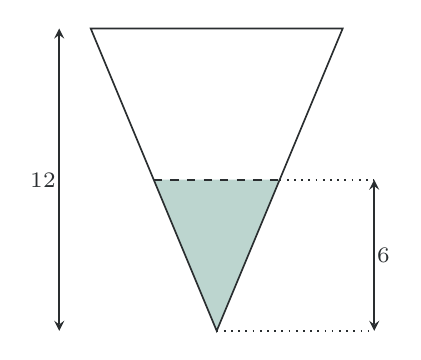
\begin{tikzpicture}[line width=0.6pt,ink,every node/.style={font=\footnotesize}]
\fill[accent!28] (0.000mm,0.000mm) -- (-8.000mm,19.200mm) -- (8.000mm,19.200mm) -- cycle;
\draw (0.000mm,0.000mm) -- (-16.000mm,38.400mm) -- (16.000mm,38.400mm) -- cycle;
\draw[dashed] (-8.000mm,19.200mm) -- (8.000mm,19.200mm);
\draw[<->,>=stealth] (-20.000mm,0.000mm) -- (-20.000mm,38.400mm) node[midway,left,inner sep=1pt] {$12$};
\draw[<->,>=stealth] (20.000mm,0.000mm) -- (20.000mm,19.200mm) node[midway,right,inner sep=1pt] {$6$};
\draw[dotted] (8.000mm,19.200mm) -- (20.000mm,19.200mm);
\draw[dotted] (0.000mm,0.000mm) -- (20.000mm,0.000mm);
\end{tikzpicture}}}
\satq{8}{A rectangular tank has a base that measures $2$ meters by $1.5$ meters. Water flows into the tank at a constant rate of $45$ liters per minute. How many minutes does it take for the water level to rise $0.3$ meter? ($1$ cubic meter $=1000$ liters)}{$200$}{$20$}{$2$}{$0.02$}
\satq{9}{The surface area of a sphere is increased by $125\%$. By what percent does the volume of the sphere increase?}{$125\%$}{$337.5\%$}{$406.25\%$}{$237.5\%$}
\satg{10}{A closed right circular cylinder has a height of $10$ and a total surface area of $192\pi$ (both circular bases and the curved side). What is the radius of the cylinder?}
\satg{11}{A circular sector with radius $10$ and central angle $288^\circ$ is cut out of paper, and its two straight edges are joined to form a right circular cone. The volume of the cone is $k\pi$. What is the value of $k$?}
}
\end{textblock*}
\begin{textblock*}{\COLW}(\RCOL,32mm)
{\fontsize{10}{12.5}\selectfont
\setkicker{Set 4 (cont.)}{Solids}
\satq{12}{A sphere fits snugly inside a right circular cylinder: it touches the top, the bottom and the curved side of the cylinder (see the figure). The volume of the cylinder is $432\pi$. What is the volume of the sphere?\figbox{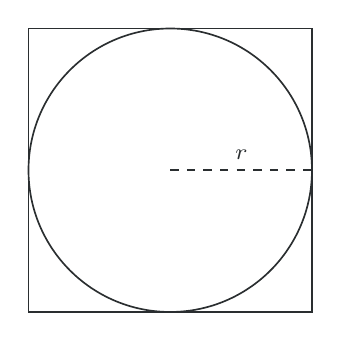
\begin{tikzpicture}[line width=0.6pt,ink,every node/.style={font=\footnotesize}]
\draw (-18.000mm,0.000mm) rectangle (18.000mm,36.000mm);
\draw (0.000mm,18.000mm) circle (18.000mm);
\draw[dashed] (0.000mm,18.000mm) -- (18.000mm,18.000mm);
\node[above=0pt] at (9.000mm,18.000mm) {$r$};
\end{tikzpicture}}}{$144 \pi$}{$216 \pi$}{$288 \pi$}{$576 \pi$}
\satq{13}{A rectangular tank has a base $40$ cm by $25$ cm and contains water to a depth of $8$ cm. A solid cube with edge length $10$ cm is placed flat on the bottom of the tank. To the nearest tenth of a centimeter, what is the new depth of the water, measured from the bottom of the tank?}{$8.9$}{$8.0$}{$9.0$}{$10.0$}
\satq{14}{A cylindrical can has a diameter of $8$ centimeters and a height of $15$ centimeters. To the nearest hundredth of a liter, how much does the can hold when full? ($1$ liter $=1000$ cubic centimeters)}{$0.19$}{$0.75$}{$3.01$}{$7.54$}
}
\end{textblock*}
\clearpage
\topicheader{8}{Hard Circles, Area \& Volume}
\pagefooter{7}
\colrule{32}{238}
\mbox{}%
\begin{textblock*}{\COLW}(\LCOL,32mm)
{\fontsize{10}{12.5}\selectfont
\setkicker{Set 5}{Summit: the hardest mixed problems.}
\satg{1}{Two parallel chords of a circle have lengths $24$ and $10$. The chords lie on opposite sides of the center of the circle, and the distance between the chords is $17$ (see the figure). What is the radius of the circle?\figbox{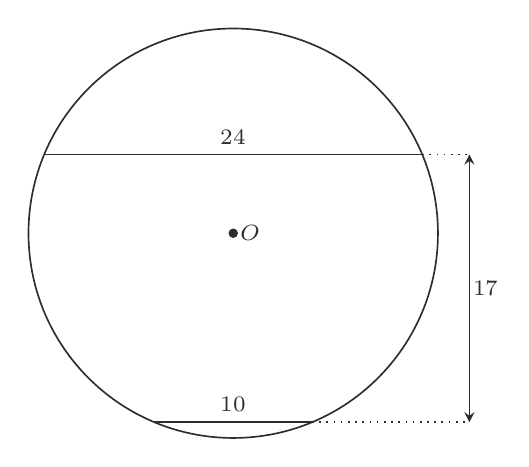
\begin{tikzpicture}[line width=0.6pt,ink,every node/.style={font=\footnotesize}]
\draw (0.000mm,0.000mm) circle (26.000mm);
\draw (-24.000mm,10.000mm) -- (24.000mm,10.000mm); \draw (-10.000mm,-24.000mm) -- (10.000mm,-24.000mm);
\fill[ink] (0.000mm,0.000mm) circle (0.6mm); \node[right,inner sep=1.5pt,xshift=1pt] at (0.000mm,0.000mm) {$O$};
\draw[dotted] (24.000mm,10.000mm) -- (30.000mm,10.000mm); \draw[dotted] (10.000mm,-24.000mm) -- (30.000mm,-24.000mm);
\draw[<->,>=stealth] (30.000mm,-24.000mm) -- (30.000mm,10.000mm) node[midway,right,inner sep=1pt] {$17$};
\node[above] at (0.000mm,10.000mm) {$24$};
\node[above] at (0.000mm,-24.000mm) {$10$};
\end{tikzpicture}}}
\satq{2}{In the first quadrant of the $xy$-plane, two different circles are each tangent to both the $x$-axis and the $y$-axis, and each passes through the point $(2,1)$. What is the sum of the areas of the two circles?}{$26 \pi$}{$25 \pi$}{$6 \pi$}{$36 \pi$}
\satg{3}{A sector of a circle has area $12$ and arc length $6$. What is the measure, in radians, of the central angle of the sector?}
}
\end{textblock*}
\begin{textblock*}{\COLW}(\RCOL,32mm)
{\fontsize{10}{12.5}\selectfont
\setkicker{Set 5 (cont.)}{Summit}
\satq{4}{Four points $A$, $B$, $C$, $D$ lie in this order on a circle so that the arcs $AB$, $BC$, $CD$ and $DA$ (the arcs between consecutive points that contain no other of the four points) are in the ratio $1:2:3:4$. Chords $\overline{AC}$ and $\overline{BD}$ intersect at point $P$ inside the circle (see the figure). What is the measure, in degrees, of $\angle APB$?\figbox{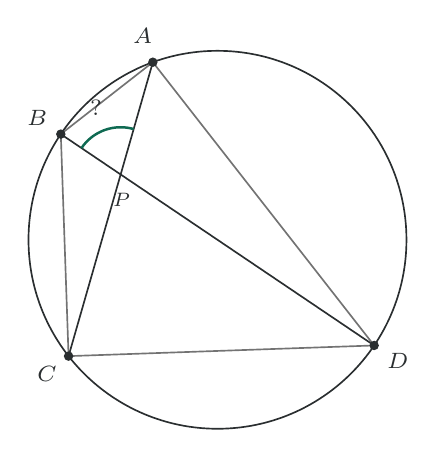
\begin{tikzpicture}[line width=0.6pt,ink,every node/.style={font=\footnotesize}]
\draw (0.000mm,0.000mm) circle (24.000mm);
\draw (-8.208mm,22.553mm) -- (-18.912mm,-14.776mm); \draw (-19.897mm,13.421mm) -- (19.897mm,-13.421mm);
\draw[black!55] (-8.208mm,22.553mm) -- (-19.897mm,13.421mm) -- (-18.912mm,-14.776mm) -- (19.897mm,-13.421mm) -- cycle;
\draw[accent,line width=0.9pt] (-10.643mm,14.062mm) arc[start angle=74.000,end angle=146.000,radius=6mm];
\node[inner sep=0pt] at (-15.375mm,16.752mm) {$?$};
\fill[ink] (-8.208mm,22.553mm) circle (0.6mm); \node[inner sep=0pt] at (-9.440mm,25.936mm) {$A$};
\fill[ink] (-19.897mm,13.421mm) circle (0.6mm); \node[inner sep=0pt] at (-22.881mm,15.434mm) {$B$};
\fill[ink] (-18.912mm,-14.776mm) circle (0.6mm); \node[inner sep=0pt] at (-21.749mm,-16.992mm) {$C$};
\fill[ink] (19.897mm,-13.421mm) circle (0.6mm); \node[inner sep=0pt] at (22.881mm,-15.434mm) {$D$};
\node[inner sep=0pt,xshift=0pt] at (-12.297mm,5.094mm) {\scriptsize $P$};
\end{tikzpicture}}}{$144^\circ$}{$108^\circ$}{$72^\circ$}{$36^\circ$}
\satq{5}{A cylindrical tank has a radius of $3$ meters and a height of $4$ meters and is initially empty. An inlet pipe adds water at a constant rate of $6\pi$ cubic meters per hour while a drain removes water at a constant rate of $2\pi$ cubic meters per hour. Both run at the same time. How many hours does it take for the tank to be completely full?}{$4.5$}{$6$}{$18$}{$9$}
\satq{6}{A solid sphere has a volume of $4500\pi$ cubic centimeters. A plane cuts the sphere at a distance of $9$ centimeters from the center of the sphere. What is the area, in square centimeters, of the circular cross-section made by the plane?}{$81 \pi$}{$144 \pi$}{$225 \pi$}{$306 \pi$}
\satq{7}{A cube has edge length $6$. A sphere passes through all $8$ vertices of the cube. What is the volume of the sphere?}{$36 \pi$}{$108 \sqrt{3} \pi$}{$72 \sqrt{2} \pi$}{$288 \pi$}
}
\end{textblock*}
\clearpage
\topicheader{8}{Hard Circles, Area \& Volume}
\pagefooter{8}
\colrule{32}{238}
\mbox{}%
\begin{textblock*}{\COLW}(\LCOL,32mm)
{\fontsize{10}{12.5}\selectfont
\setkicker{Set 5 (cont.)}{Summit}
\satg{8}{Two similar solids have surface areas of $18$ and $50$. The volume of the smaller solid is $54$. What is the volume of the larger solid?}
\satqw{9}{The radius of a right circular cylinder is increased by $10\%$ and its height is decreased by $20\%$. Which of the following describes the change in the volume of the cylinder?}{Decreases by $12\%$}{Decreases by $10\%$}{Decreases by $3.2\%$}{Does not change}
\satq{10}{In the $xy$-plane, a circle has equation $x^2+y^2-4x-6y-12=0$. Point $P$ has coordinates $(15,3)$ and lies outside the circle. A line through $P$ touches the circle at exactly one point $T$. What is the length of $\overline{PT}$?}{$12$}{$5$}{$8$}{$13$}
\satg{11}{A circle in the $xy$-plane passes through the points $(0,0)$, $(12,0)$ and $(0,5)$. What is the radius of the circle?}
\satq{12}{A silo is a right circular cylinder with a hemisphere on top (see the figure). The base radius is $4$ feet, and the total height of the silo, from the ground to the top of the hemisphere, is $10$ feet. What is the volume of the silo, in cubic feet?\figbox{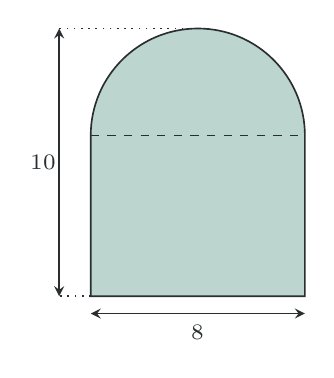
\begin{tikzpicture}[line width=0.6pt,ink,every node/.style={font=\footnotesize}]
\fill[accent!28] (-13.600mm,0.000mm) -- (13.600mm,0.000mm) -- (13.600mm,20.400mm) arc[start angle=0,end angle=180,radius=13.600mm] -- cycle;
\draw (-13.600mm,0.000mm) -- (13.600mm,0.000mm) -- (13.600mm,20.400mm) arc[start angle=0,end angle=180,radius=13.600mm] -- cycle;
\draw[dashed] (-13.600mm,20.400mm) -- (13.600mm,20.400mm);
\draw[<->,>=stealth] (-17.600mm,0.000mm) -- (-17.600mm,34.000mm) node[midway,left,inner sep=1pt] {$10$};
\draw[dotted] (-13.600mm,0.000mm) -- (-17.600mm,0.000mm); \draw[dotted] (0.000mm,34.000mm) -- (-17.600mm,34.000mm);
\draw[<->,>=stealth] (-13.600mm,-2.200mm) -- (13.600mm,-2.200mm) node[midway,below=0.5pt] {$8$};
\end{tikzpicture}}}{$224 \pi$}{$\frac{608 \pi}{3}$}{$\frac{544 \pi}{3}$}{$\frac{416 \pi}{3}$}
}
\end{textblock*}
\begin{textblock*}{\COLW}(\RCOL,32mm)
{\fontsize{10}{12.5}\selectfont
\setkicker{Set 5 (cont.)}{Summit}
\satq{13}{A cylindrical can with a radius of $10$ cm holds water to a depth of $9$ cm. All of the water is poured into an empty rectangular box whose base measures $15$ cm by $12$ cm. What is the depth, in cm, of the water in the box?}{$50 \pi$}{$20 \pi$}{$5 \pi$}{$5$}
\satq{14}{A circle has radius $9$. The minor arc $AB$ has length $6\pi$. What is the length of chord $\overline{AB}$?}{$9 \sqrt{3}$}{$9$}{$9 \sqrt{2}$}{$18$}
\satg{15}{A regular hexagon with side length $6$ is inscribed in a circle (all six vertices lie on the circle). The area of the region inside the circle but outside the hexagon is $a\pi-b\sqrt3$. What is the value of $a+b$?}
\satq{16}{A pyramid has a square base with side length $12$ and a height of $9$; its apex is directly above the center of the base. A plane parallel to the base cuts the pyramid at a height of $3$ above the base (see the figure). What is the area of the cross-section?\figbox{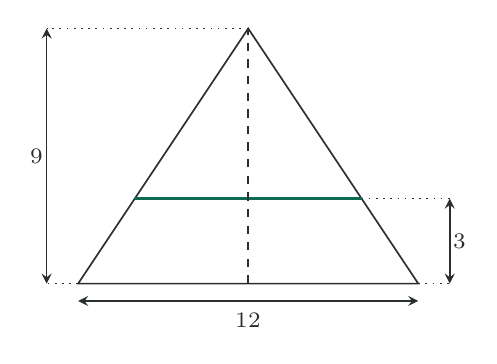
\begin{tikzpicture}[line width=0.6pt,ink,every node/.style={font=\footnotesize}]
\draw (-21.600mm,0.000mm) -- (21.600mm,0.000mm) -- (0.000mm,32.400mm) -- cycle;
\draw[accent,line width=1.2pt] (-14.400mm,10.800mm) -- (14.400mm,10.800mm);
\draw[dashed] (0.000mm,0.000mm) -- (0.000mm,32.400mm);
\draw[<->,>=stealth] (-21.600mm,-2.200mm) -- (21.600mm,-2.200mm) node[midway,below=0.5pt] {$12$};
\draw[<->,>=stealth] (-25.600mm,0.000mm) -- (-25.600mm,32.400mm) node[midway,left,inner sep=1pt] {$9$};
\draw[dotted] (-21.600mm,0.000mm) -- (-25.600mm,0.000mm); \draw[dotted] (0.000mm,32.400mm) -- (-25.600mm,32.400mm);
\draw[<->,>=stealth] (25.600mm,0.000mm) -- (25.600mm,10.800mm) node[midway,right,inner sep=1pt] {$3$};
\draw[dotted] (14.400mm,10.800mm) -- (25.600mm,10.800mm);
\draw[dotted] (21.600mm,0.000mm) -- (25.600mm,0.000mm);
\end{tikzpicture}}}{$8$}{$64$}{$16$}{$96$}
\satg{17}{A right circular cone has height $12$. A plane parallel to the base cuts off a small cone at the top; the plane is $4$ units below the apex. The small cone has volume $8\pi$. The remaining solid (the frustum) has volume $k\pi$. What is the value of $k$?}
}
\end{textblock*}
\clearpage
\topicheader{8}{Hard Circles, Area \& Volume}
\pagefooter{9}
\colrule{32}{238}
\mbox{}%
\begin{textblock*}{\COLW}(\LCOL,32mm)
{\fontsize{10}{12.5}\selectfont
\setkicker{Set 5 (cont.)}{Summit}
\satq{18}{A container is an inverted right circular cone (point down) with top radius $6$ cm and height $9$ cm. It is initially empty and water flows in at a constant rate of $12\pi$ cubic centimeters per minute. How many minutes does it take for the water depth to reach $4.5$ cm?}{$13.5$}{$9$}{$4.5$}{$1.125$}
\satq{19}{Two circles have the same center and radii $4$ and $10$. Two radii of the larger circle form an angle of $72^\circ$. What is the area of the part of the region between the two circles that lies inside this $72^\circ$ angle?}{$\frac{12 \pi}{5}$}{$\frac{36 \pi}{5}$}{$\frac{84 \pi}{5}$}{$84 \pi$}
\satq{20}{A sector of a circle has an area of $36$ and a central angle of $2$ radians. What is the perimeter of the sector (the arc length plus the two straight edges)?}{$12$}{$18$}{$24$}{$36$}
}
\end{textblock*}
\clearpage
\topicheader{8}{Hard Circles, Area \& Volume}
\pagefooter{10}
\mbox{}%
\begin{textblock*}{178mm}(16mm,30mm)
{\bfseries\itshape\color{accent}\fontsize{19}{21}\selectfont\centering Answer Key\par}
\end{textblock*}
\begin{textblock*}{178mm}(16mm,41mm)
{\fontsize{9.5}{12}\selectfont\color{black!70}\centering Multiple choice: the letter. Grid-in: the number to enter. Worked solutions follow on the next pages.\par}
\end{textblock*}
\begin{textblock*}{178mm}(16mm,52mm)
{\fontsize{10}{13}\selectfont
\centering
\setlength{\tabcolsep}{2pt}\renewcommand{\arraystretch}{1.3}
{\sffamily\bfseries\color{accent}\fontsize{11}{13}\selectfont Set 1 \ \textmd{\itshape\small Bridge: the core moves}}\\[1.3mm]
\begin{tabular}{|>{\centering\arraybackslash}p{16mm}|>{\centering\arraybackslash}p{16mm}|>{\centering\arraybackslash}p{16mm}|>{\centering\arraybackslash}p{16mm}|>{\centering\arraybackslash}p{16mm}|>{\centering\arraybackslash}p{16mm}|>{\centering\arraybackslash}p{16mm}|>{\centering\arraybackslash}p{16mm}|>{\centering\arraybackslash}p{16mm}|>{\centering\arraybackslash}p{16mm}|}
\hline
\cellcolor{badge!55}\textbf{1} & \cellcolor{badge!55}\textbf{2} & \cellcolor{badge!55}\textbf{3} & \cellcolor{badge!55}\textbf{4} & \cellcolor{badge!55}\textbf{5} & \cellcolor{badge!55}\textbf{6} & \cellcolor{badge!55}\textbf{7} & \cellcolor{badge!55}\textbf{8} & \cellcolor{badge!55}\textbf{9} & \cellcolor{badge!55}\textbf{10}\\
\hline
\textbf{B} & \textbf{A} & 4 & \textbf{D} & \textbf{A} & \textbf{C} & \textbf{C} & \textbf{B} & 60 & \textbf{D}\\
\hline
\end{tabular}\\[1.5mm]
\begin{tabular}{|>{\centering\arraybackslash}p{16mm}|>{\centering\arraybackslash}p{16mm}|}
\hline
\cellcolor{badge!55}\textbf{11} & \cellcolor{badge!55}\textbf{12}\\
\hline
\textbf{B} & 4\\
\hline
\end{tabular}\\[1.5mm]
\vspace{3.5mm}
{\sffamily\bfseries\color{accent}\fontsize{11}{13}\selectfont Set 2 \ \textmd{\itshape\small Circles: equations, tangents, chords, angles, arcs}}\\[1.3mm]
\begin{tabular}{|>{\centering\arraybackslash}p{16mm}|>{\centering\arraybackslash}p{16mm}|>{\centering\arraybackslash}p{16mm}|>{\centering\arraybackslash}p{16mm}|>{\centering\arraybackslash}p{16mm}|>{\centering\arraybackslash}p{16mm}|>{\centering\arraybackslash}p{16mm}|>{\centering\arraybackslash}p{16mm}|>{\centering\arraybackslash}p{16mm}|>{\centering\arraybackslash}p{16mm}|}
\hline
\cellcolor{badge!55}\textbf{1} & \cellcolor{badge!55}\textbf{2} & \cellcolor{badge!55}\textbf{3} & \cellcolor{badge!55}\textbf{4} & \cellcolor{badge!55}\textbf{5} & \cellcolor{badge!55}\textbf{6} & \cellcolor{badge!55}\textbf{7} & \cellcolor{badge!55}\textbf{8} & \cellcolor{badge!55}\textbf{9} & \cellcolor{badge!55}\textbf{10}\\
\hline
\textbf{A} & 8 & \textbf{C} & \textbf{A} & 9 & \textbf{B} & \textbf{C} & 4 & \textbf{A} & \textbf{D}\\
\hline
\end{tabular}\\[1.5mm]
\begin{tabular}{|>{\centering\arraybackslash}p{16mm}|>{\centering\arraybackslash}p{16mm}|>{\centering\arraybackslash}p{16mm}|>{\centering\arraybackslash}p{16mm}|}
\hline
\cellcolor{badge!55}\textbf{11} & \cellcolor{badge!55}\textbf{12} & \cellcolor{badge!55}\textbf{13} & \cellcolor{badge!55}\textbf{14}\\
\hline
\textbf{B} & \textbf{D} & 5 & \textbf{D}\\
\hline
\end{tabular}\\[1.5mm]
\vspace{3.5mm}
{\sffamily\bfseries\color{accent}\fontsize{11}{13}\selectfont Set 3 \ \textmd{\itshape\small Areas: shaded, composite, scaling}}\\[1.3mm]
\begin{tabular}{|>{\centering\arraybackslash}p{16mm}|>{\centering\arraybackslash}p{16mm}|>{\centering\arraybackslash}p{16mm}|>{\centering\arraybackslash}p{16mm}|>{\centering\arraybackslash}p{16mm}|>{\centering\arraybackslash}p{16mm}|>{\centering\arraybackslash}p{16mm}|>{\centering\arraybackslash}p{16mm}|>{\centering\arraybackslash}p{16mm}|>{\centering\arraybackslash}p{16mm}|}
\hline
\cellcolor{badge!55}\textbf{1} & \cellcolor{badge!55}\textbf{2} & \cellcolor{badge!55}\textbf{3} & \cellcolor{badge!55}\textbf{4} & \cellcolor{badge!55}\textbf{5} & \cellcolor{badge!55}\textbf{6} & \cellcolor{badge!55}\textbf{7} & \cellcolor{badge!55}\textbf{8} & \cellcolor{badge!55}\textbf{9} & \cellcolor{badge!55}\textbf{10}\\
\hline
\textbf{D} & \textbf{C} & \textbf{B} & 216 & \textbf{A} & \textbf{D} & \textbf{C} & 30 & \textbf{B} & \textbf{C}\\
\hline
\end{tabular}\\[1.5mm]
\begin{tabular}{|>{\centering\arraybackslash}p{16mm}|>{\centering\arraybackslash}p{16mm}|>{\centering\arraybackslash}p{16mm}|>{\centering\arraybackslash}p{16mm}|}
\hline
\cellcolor{badge!55}\textbf{11} & \cellcolor{badge!55}\textbf{12} & \cellcolor{badge!55}\textbf{13} & \cellcolor{badge!55}\textbf{14}\\
\hline
4 & \textbf{B} & 1.44 & \textbf{D}\\
\hline
\end{tabular}\\[1.5mm]
\vspace{3.5mm}
{\sffamily\bfseries\color{accent}\fontsize{11}{13}\selectfont Set 4 \ \textmd{\itshape\small Solids: volume, surface area, filling, recasting}}\\[1.3mm]
\begin{tabular}{|>{\centering\arraybackslash}p{16mm}|>{\centering\arraybackslash}p{16mm}|>{\centering\arraybackslash}p{16mm}|>{\centering\arraybackslash}p{16mm}|>{\centering\arraybackslash}p{16mm}|>{\centering\arraybackslash}p{16mm}|>{\centering\arraybackslash}p{16mm}|>{\centering\arraybackslash}p{16mm}|>{\centering\arraybackslash}p{16mm}|>{\centering\arraybackslash}p{16mm}|}
\hline
\cellcolor{badge!55}\textbf{1} & \cellcolor{badge!55}\textbf{2} & \cellcolor{badge!55}\textbf{3} & \cellcolor{badge!55}\textbf{4} & \cellcolor{badge!55}\textbf{5} & \cellcolor{badge!55}\textbf{6} & \cellcolor{badge!55}\textbf{7} & \cellcolor{badge!55}\textbf{8} & \cellcolor{badge!55}\textbf{9} & \cellcolor{badge!55}\textbf{10}\\
\hline
\textbf{A} & \textbf{A} & 2.25 & \textbf{C} & \textbf{B} & \textbf{C} & 12.5 & \textbf{B} & \textbf{D} & 6\\
\hline
\end{tabular}\\[1.5mm]
\begin{tabular}{|>{\centering\arraybackslash}p{16mm}|>{\centering\arraybackslash}p{16mm}|>{\centering\arraybackslash}p{16mm}|>{\centering\arraybackslash}p{16mm}|}
\hline
\cellcolor{badge!55}\textbf{11} & \cellcolor{badge!55}\textbf{12} & \cellcolor{badge!55}\textbf{13} & \cellcolor{badge!55}\textbf{14}\\
\hline
128 & \textbf{C} & \textbf{A} & \textbf{B}\\
\hline
\end{tabular}\\[1.5mm]
\vspace{3.5mm}
{\sffamily\bfseries\color{accent}\fontsize{11}{13}\selectfont Set 5 \ \textmd{\itshape\small Summit: the hardest mixed problems}}\\[1.3mm]
\begin{tabular}{|>{\centering\arraybackslash}p{16mm}|>{\centering\arraybackslash}p{16mm}|>{\centering\arraybackslash}p{16mm}|>{\centering\arraybackslash}p{16mm}|>{\centering\arraybackslash}p{16mm}|>{\centering\arraybackslash}p{16mm}|>{\centering\arraybackslash}p{16mm}|>{\centering\arraybackslash}p{16mm}|>{\centering\arraybackslash}p{16mm}|>{\centering\arraybackslash}p{16mm}|}
\hline
\cellcolor{badge!55}\textbf{1} & \cellcolor{badge!55}\textbf{2} & \cellcolor{badge!55}\textbf{3} & \cellcolor{badge!55}\textbf{4} & \cellcolor{badge!55}\textbf{5} & \cellcolor{badge!55}\textbf{6} & \cellcolor{badge!55}\textbf{7} & \cellcolor{badge!55}\textbf{8} & \cellcolor{badge!55}\textbf{9} & \cellcolor{badge!55}\textbf{10}\\
\hline
13 & \textbf{A} & 1.5 & \textbf{C} & \textbf{D} & \textbf{B} & \textbf{B} & 250 & \textbf{C} & \textbf{A}\\
\hline
\end{tabular}\\[1.5mm]
\begin{tabular}{|>{\centering\arraybackslash}p{16mm}|>{\centering\arraybackslash}p{16mm}|>{\centering\arraybackslash}p{16mm}|>{\centering\arraybackslash}p{16mm}|>{\centering\arraybackslash}p{16mm}|>{\centering\arraybackslash}p{16mm}|>{\centering\arraybackslash}p{16mm}|>{\centering\arraybackslash}p{16mm}|>{\centering\arraybackslash}p{16mm}|>{\centering\arraybackslash}p{16mm}|}
\hline
\cellcolor{badge!55}\textbf{11} & \cellcolor{badge!55}\textbf{12} & \cellcolor{badge!55}\textbf{13} & \cellcolor{badge!55}\textbf{14} & \cellcolor{badge!55}\textbf{15} & \cellcolor{badge!55}\textbf{16} & \cellcolor{badge!55}\textbf{17} & \cellcolor{badge!55}\textbf{18} & \cellcolor{badge!55}\textbf{19} & \cellcolor{badge!55}\textbf{20}\\
\hline
6.5 & \textbf{D} & \textbf{C} & \textbf{A} & 90 & \textbf{B} & 208 & \textbf{D} & \textbf{C} & \textbf{C}\\
\hline
\end{tabular}\\[1.5mm]
\vspace{3.5mm}
}
\end{textblock*}
\clearpage
%%AUTOFLOW-SOLUTIONS
\newgeometry{top=34mm,bottom=24mm,left=16mm,right=16mm}
\pagestyle{solstyle}
\setlength{\columnsep}{14mm}\setlength{\columnseprule}{0.4pt}
{\fontsize{10}{13.6}\selectfont
\begin{multicols}{2}
\solkitem{Set 1}{1}{B ($12$)}{The right side is $r^2=36$, so $r=6$ and the diameter is $2r=12$. ($6$ is the radius; $36$ is $r^2$; $72$ doubles $r^2$.)}{Read $r^2$, then double $r$}
\solitem{2}{A $(3,0)$}{A point is inside when $(x-1)^2+(y+2)^2<25$. For $(3,0)$: $4+4=8<25$. ($(-3,-5)$ gives $16+9=25$ and $(1,3)$ gives $0+25=25$: both are \emph{on} the circle; $(6,1)$ gives $25+9=34>25$, outside.)}{Compare distance$^2$ with $r^2$}
\solitem{3}{Ans. 4}{The arc is $\frac{80}{360}=\frac29$ of the circumference $2\pi(9)=18\pi$, so it is $\frac29\cdot18\pi=4\pi$ and $k=4$.}{Arc = fraction of the circumference}
\solitem{4}{D ($150$)}{The radius is $12$, so the circle has area $144\pi$ and the sector is $\frac{60\pi}{144\pi}=\frac5{12}$ of it: $\frac5{12}(360^\circ)=150^\circ$. ($37.5$ uses the diameter $24$ as the radius; $60$ copies the coefficient; $75$ uses $180^\circ$ for the full turn.)}{Sector = $\frac{\theta}{360}\pi r^2$ with $r=\frac d2$}
\solitem{5}{A ($50^\circ$)}{An inscribed angle is half the central angle on the same arc: $\frac{100}2=50^\circ$. ($100$ is the central angle; $130$ is the answer if $C$ were on the minor arc, $180-50$; $200$ doubles instead of halving.)}{Inscribed angle = half the central angle}
\solitem{6}{C ($144 \pi$)}{$\frac43\pi r^3=288\pi$ gives $r^3=216$, $r=6$. Then $4\pi r^2=4\pi(36)=144\pi$. ($36\pi$ is $\pi r^2$; $72\pi$ is $2\pi r^2$; $576\pi$ uses the diameter $12$ as the radius.)}{Volume gives $r$; surface area is $4\pi r^2$}
\solitem{7}{C ($2{,}400$)}{$V=2(1.5)(0.8)=2.4$ m$^3$, and $2.4\times1000=2400$ L. ($2.4$ forgets the conversion; $240$ and $24{,}000$ slip the decimal point.)}{Cubic meters $\to$ liters: $\times1000$}
\solitem{8}{B ($1{,}080$)}{Lengths scale by $k=3$, so volume scales by $k^3=27$: $40\times27=1080$. ($120$ multiplies by $3$; $360$ by $k^2=9$; $3{,}240$ by $3^4$.)}{Scale factor $k$: volume $\times k^3$}
\solitem{9}{Ans. 60}{The circumference is $2\pi(6)=12\pi$, so the arc is $\frac{2\pi}{12\pi}=\frac16$ of the circle and $\theta=\frac16(360)=60^\circ$.}{Arc $\div$ circumference $=\frac{\theta}{360}$}
\solitem{10}{D ($60 + \frac{9 \pi}{2}$)}{The semicircle has diameter $6$, so $r=3$ and its area is $\frac12\pi(3)^2=\frac92\pi$. Total $60+\frac92\pi$. ($60+9\pi$ is a full circle; $60+18\pi$ is a semicircle of radius $6$; $60+36\pi$ is a full circle of radius $6$.)}{Semicircle: $\frac12\pi r^2$ with $r=\frac d2$}
\solitem{11}{B ($1.5$)}{Each minute the volume added is $\pi r^2\cdot(\text{rise})$: $24\pi=16\pi\cdot\text{rise}$, so the rise is $1.5$ ft. ($3$ divides by the circumference $8\pi$; $6$ divides by $r$; $0.375$ divides by $r^3$.)}{Rate $=$ (base area)(rise per minute)}
\solitem{12}{Ans. 4}{$(x^2-6x+9)+(y^2+10y+25)=-18+9+25$, so $(x-3)^2+(y+5)^2=16$ and $r=\sqrt{16}=4$. (Moving $18$ to the right gives $-18$, not $+18$; and $16$ is $r^2$.)}{Complete the square, then watch the constant}
\solkitem{Set 2}{1}{A ($-8$)}{$(x+4)^2+(y-1)^2=17-k$, and this must equal $r^2=25$, so $k=17-25=-8$. ($8$ drops the sign; $12$ uses $r=5$ instead of $r^2$; $42=17+25$.)}{Complete the square: $r^2=h^2+k^2-c$}
\solitem{2}{Ans. 8}{On the $x$-axis $y=0$, so $x^2-4x-12=0$, i.e. $(x-6)(x+2)=0$. The points are $x=6$ and $x=-2$, which are $8$ apart.}{Set $y=0$ to find axis crossings}
\solitem{3}{C $(9,0)$}{The radius from $(2,-1)$ to $(5,3)$ has slope $\frac43$, so the tangent has slope $-\frac34$: $y-3=-\frac34(x-5)$. At $x=9$: $y=3-3=0$. ($(8,7)$ has slope $\frac43$, parallel to the radius; $(9,6)$ has slope $+\frac34$; $(8,-1)$ has slope $-\frac43$.)}{Tangent $\perp$ radius: negative reciprocal slope}
\solitem{4}{A ($64$)}{The center is the origin, whose distance to $3x-4y-40=0$ is $\frac{|{-40}|}{\sqrt{3^2+4^2}}=8$. That distance is the radius, and $k=r^2=64$. ($8$ is $r$; $40$ and $1600$ ignore the $\sqrt{3^2+4^2}$.)}{Tangent $\Rightarrow$ distance from center to line $=r$}
\solitem{5}{Ans. 9}{$OM\perp AB$ and $AM=15$, so $OM=\sqrt{17^2-15^2}=8$. Then $MN=ON-OM=17-8=9$. (The common error is to stop at $8$, the distance from the center to the chord.)}{Perpendicular from the center bisects the chord}
\solitem{6}{B ($124$)}{$\angle ACB=90^\circ$ (angle in a semicircle), so $\angle ABC=180-90-28=62^\circ$. Arc $AC$ is intercepted by $\angle ABC$: $2(62)=124^\circ$. ($56$ is arc $BC$; $62$ is the inscribed angle itself; $152=180-28$.)}{Semicircle $\Rightarrow90^\circ$, then arc $=2\times$ inscribed angle}
\solitem{7}{C ($65^\circ$)}{In quadrilateral $OAEU$ the angles at $A$ and $U$ are $90^\circ$, so $\angle AOU=360-90-90-50=130^\circ$. The inscribed angle on the major arc is half of it: $65^\circ$. ($130$ is the central angle; $115=180-65$ is for $C$ on the minor arc; $50$ is given.)}{Kite $OAEU$: two right angles, then half the central angle}
\solitem{8}{Ans. 4}{$\angle OAE=90^\circ$, so $OE=\sqrt{6^2+8^2}=10$. Then $PE=OE-OP=10-6=4$. (A frequent slip is to answer $10$, the distance $OE$ itself.)}{Tangent $\perp$ radius: $OE^2=r^2+t^2$}
\solitem{9}{A ($4 \pi$)}{$\frac{60}{360}\pi r^2=24\pi$ gives $r^2=144$, $r=12$. Arc $=\frac16(2\pi\cdot12)=4\pi$. ($24\pi$ is the whole circumference; $12\pi$ is $\pi r$; $2\pi$ halves the arc.)}{Area $\to r$, then arc $=\frac{\theta}{360}\cdot2\pi r$}
\solitem{10}{D ($\frac{135 \pi}{4}$)}{With $\theta$ in radians, $A=\frac12r^2\theta=\frac12(81)\cdot\frac{5\pi}6=\frac{135\pi}{4}$. ($\frac{135\pi}2$ forgets the $\frac12$; $\frac{15\pi}2$ is the arc length $r\theta$; $\frac{15\pi}4$ uses $r$ instead of $r^2$.)}{Radians: area $=\frac12r^2\theta$}
\solitem{11}{B ($54 - 9 \pi$)}{The hypotenuse is $15$, the area is $54$ and the semiperimeter is $18$, so $r=\frac{54}{18}=3$. Shaded area $=54-\pi(3)^2=54-9\pi$. ($54-3\pi$ uses $r$; $54-6\pi$ uses the circumference; $54-36\pi$ uses $d=6$ as the radius.)}{Inradius $=\dfrac{\text{area}}{\text{semiperimeter}}$}
\solitem{12}{D ($64$)}{The radius is the vertical distance from $(-4,6)$ to $y=-2$: $6-(-2)=8$. So $k=r^2=64$. ($8$ is $r$; $36$ is tangent to the $x$-axis instead; $16$ uses $6-2=4$.)}{Tangent to a horizontal line: $r=|k_{\text{center}}-\text{line}|$}
\solitem{13}{Ans. 5}{Center $=(5,5)$; $r^2=\frac{8^2+6^2}{4}=25$. So $(x-5)^2+(y-5)^2=25$, i.e. $x^2+y^2-10x-10y+25=0$. Then $a+b+c=-10-10+25=5$. (The constant term is $25$, not $25-25=0$.)}{Midpoint $=$ center, half the distance $=r$}
\solitem{14}{D ($6$)}{Write the line as $x-y+k=0$. Its distance from the origin is $\frac{|k|}{\sqrt2}$, which must equal $r=\sqrt{18}=3\sqrt2$. So $|k|=6$. ($3\sqrt2$ forgets the $\sqrt2$ in the distance; $18$ is $r^2$; $9$ is half of $18$.)}{Tangent: distance from center to line $=r$}
\solkitem{Set 3}{1}{D ($144 \pi$)}{At the tangent point the radius is perpendicular to the chord and bisects it, so $R^2=r^2+12^2$. Ring area $=\pi R^2-\pi r^2=\pi(12^2)=144\pi$, whatever $r$ is. ($12\pi$ forgets to square; $288\pi$ and $576\pi$ use $24^2$ with a factor slip.)}{Half-chord is the leg of a right triangle: $R^2-r^2=(\text{half-chord})^2$}
\solitem{2}{C ($400 - 100 \pi$)}{Along one side, two circles fit across: $4r=20$, so $r=5$. Circles total $4\pi(5)^2=100\pi$; shaded area $=400-100\pi$. ($400-25\pi$ counts one circle; $400-40\pi$ uses circumferences; $400-400\pi$ takes $r=10$.)}{Side $=4r$ when two circles span it}
\solitem{3}{B ($192 + 16 \pi$)}{With short side $w$: perimeter $=2(3w)+\pi w=(6+\pi)w=48+8\pi$, so $w=8$. Area $=24\cdot8+\pi(4)^2=192+16\pi$. ($192+8\pi$ counts one semicircle; $192+32\pi$ and $192+64\pi$ use $r=8$.)}{Two semicircles $=$ one circle; perimeter fixes the width}
\solitem{4}{Ans. 216}{The two quarter-circles together cover the square once and the lens twice, so lens $=2\left(\frac14\pi\cdot12^2\right)-12^2=72\pi-144$. Hence $a=72$, $b=144$ and $a+b=216$.}{Overlap $=$ two quarter-circles $-$ the square}
\solitem{5}{A ($50 \pi - 100$)}{The diagonal $10\sqrt2$ is the diameter, so $r=5\sqrt2$ and the circle has area $\pi(50)=50\pi$. Subtract the square: $50\pi-100$. ($50\pi$ forgets to subtract; $100\pi-100$ takes $r=10$; $200\pi-100$ takes $r=10\sqrt2$.)}{Diagonal of the square $=$ diameter}
\solitem{6}{D ($36\%$)}{Let the small radius be $1$ and the large one $1.25$. Areas: $1$ and $1.5625$. Ring share $=\frac{1.5625-1}{1.5625}=0.36$, i.e. $36\%$. ($64\%$ is the inner disk; $56.25\%$ compares the ring with the inner disk; $25\%$ is the radius change.)}{Areas go with $(\text{radius})^2$}
\solitem{7}{C ($6 \pi - 9 \sqrt{3}$)}{Sector: $\frac16\pi(36)=6\pi$. Triangle $OAB$ is equilateral with side $6$: area $\frac{\sqrt3}{4}(36)=9\sqrt3$. Segment $=6\pi-9\sqrt3$. ($6\pi$ is the sector alone; $6\pi-9$ drops the $\sqrt3$; $6\pi-18\sqrt3$ doubles the triangle.)}{Segment $=$ sector $-$ triangle}
\solitem{8}{Ans. 30}{$(1+\frac p{100})^2=1.69$, so $1+\frac p{100}=1.3$ and $p=30$. (Halving $69$ to get $34.5$ ignores the squaring.)}{Area factor $=(\text{radius factor})^2$}
\solitem{9}{B ($12 \pi$)}{The center is also the centroid, at distance $\frac23$ of the altitude $3\sqrt3$ from a vertex: $r=2\sqrt3$. Area $=\pi(2\sqrt3)^2=12\pi$. ($3\pi$ uses the inradius $\sqrt3$; $9\pi$ uses $r=3$; $36\pi$ uses $r=6$.)}{Circumradius of an equilateral triangle $=\frac{a}{\sqrt3}$}
\solitem{10}{C ($12$)}{Draw a segment from $O_1$ parallel to $PQ$. It forms a right triangle with hypotenuse $O_1O_2=4+9=13$ and one leg $9-4=5$, so $PQ=\sqrt{13^2-5^2}=12$. ($13$ is the center distance; $5$ is the radius difference; $6=\sqrt{4\cdot9}$ forgets the factor $2$.)}{Common tangent: right triangle with legs $PQ$ and $r_2-r_1$}
\solitem{11}{Ans. 4}{Radii $2k$ and $3k$: $\pi(4k^2+9k^2)=13\pi k^2=52\pi$, so $k=2$ and the smaller radius is $2k=4$. (Not $k=2$, and not $6$, the larger radius.)}{Ratio $2k:3k$, then add the squares}
\solitem{12}{B ($100 \pi - 192$)}{The diagonal is $\sqrt{16^2+12^2}=20$, so $r=10$ and the circle has area $100\pi$. Subtract $16\cdot12=192$. ($64\pi-192$ uses half the long side as $r$; $100\pi-96$ subtracts half the rectangle; $400\pi-192$ uses the diagonal as $r$.)}{Diagonal of the rectangle $=$ diameter}
\solitem{13}{Ans. 1.44}{$240$ cm $=2.4$ m, so $r=1.2$ m and the area is $\pi(1.2)^2=1.44\pi$ m$^2$. (Using $1\ \text{m}^2=100\ \text{cm}^2$ would give $144$.)}{Convert length first, then square}
\solitem{14}{D ($2$)}{For side $s$: $r_A=\frac s2$ and $r_B=\frac{s\sqrt2}2$, so $r_B=\sqrt2\,r_A$. Areas scale with the square: $(\sqrt2)^2=2$. ($\sqrt2$ is the radius ratio; $4$ squares twice; $2\sqrt2$ cubes.)}{Radius ratio $\sqrt2$, area ratio $(\sqrt2)^2$}
\solkitem{Set 4}{1}{A ($10$)}{$\pi(5^2)(12)=\pi r^2(3)$ gives $r^2=100$ and $r=10$. (The height drops by a factor of $4$, so the radius \emph{doubles}, not $\times4$ ($20$); $25$ is $r_1^2$; $100$ is $r_2^2$.)}{Equal volumes: $r^2h$ matches, so $r^2$ scales like $1/h$}
\solitem{2}{A ($100 \pi$)}{$r=5$, so $h=\sqrt{13^2-5^2}=12$ and $V=\frac13\pi(25)(12)=100\pi$. ($300\pi$ forgets the $\frac13$; $\frac{325\pi}3$ uses the slant height $13$ as $h$; $\frac{1300\pi}3$ also uses $r=10$.)}{Slant height is not the height: $h=\sqrt{l^2-r^2}$}
\solitem{3}{Ans. 2.25}{The sphere displaces $\frac43\pi(3)^3=36\pi$ dm$^3$. This equals $\pi(4)^2\cdot h$, so $h=\frac{36}{16}=2.25$.}{Displaced volume $=$ base area $\times$ rise}
\solitem{4}{C ($27$)}{Cylinder: $\pi(36)(8)=288\pi$. One sphere: $\frac43\pi(8)=\frac{32\pi}3$. Number $=288\pi\div\frac{32\pi}3=27$. ($9$ forgets the $\frac13$; $36$ uses $\pi r^3$; $54$ uses $\frac43\pi r^2$.)}{Volume is conserved: divide total by one piece}
\solitem{5}{B ($1{,}500$)}{Real lengths are $50$ times the model's, so real areas are $50^2=2500$ times: $0.6\times2500=1500$ m$^2$. ($30$ multiplies by $50$; $75{,}000$ by $50^3$; $0.012$ divides by $50$.)}{Areas scale by $k^2$}
\solitem{6}{C ($360$)}{Each face has height $\sqrt{12^2+5^2}=13$ (slant height), so its area is $\frac12(10)(13)=65$. Total $=100+4(65)=360$. ($260$ omits the base; $340$ uses $12$ as the face height; $620$ drops the $\frac12$.)}{Face height is the slant height $\sqrt{h^2+(\frac s2)^2}$}
\solitem{7}{Ans. 12.5}{The water forms a smaller cone similar to the container with scale factor $\frac12$, so its volume is $(\frac12)^3=\frac18=12.5\%$ of the whole, not $50\%$.}{Half the height is $k=\frac12$: volume $\times k^3$}
\solitem{8}{B ($20$)}{Volume needed: $2(1.5)(0.3)=0.9$ m$^3=900$ L. Time $=\frac{900}{45}=20$ min. ($0.02$ leaves the volume in m$^3$; $2$ and $200$ slip a factor of $10$.)}{Convert to one unit before dividing}
\solitem{9}{D ($237.5\%$)}{Area factor $2.25=k^2$, so $k=1.5$. Volume factor $k^3=3.375$, an increase of $237.5\%$. ($125\%$ copies the area change; $337.5\%$ is the factor, not the increase; $406.25\%$ squares $2.25$.)}{Area $\times k^2$, volume $\times k^3$: $k=\sqrt{\text{area factor}}$}
\solitem{10}{Ans. 6}{$2\pi r^2+2\pi r(10)=192\pi\Rightarrow r^2+10r-96=0\Rightarrow(r+16)(r-6)=0$. A radius is positive, so $r=6$. (Dropping the two bases gives $9.6$; $16$ is the negative root's size.)}{Surface area gives a quadratic in $r$}
\solitem{11}{Ans. 128}{The arc is $\frac{288}{360}(2\pi\cdot10)=16\pi$, which is the base circumference $2\pi r$, so $r=8$. The slant height is $10$, so $h=\sqrt{100-64}=6$. $V=\frac13\pi(64)(6)=128\pi$.}{Sector radius becomes the slant height; arc becomes the base circumference}
\solitem{12}{C ($288 \pi$)}{The cylinder has height $2r$: $\pi r^2(2r)=2\pi r^3=432\pi$, so $r^3=216$. Sphere $=\frac43\pi r^3=288\pi$, which is $\frac23$ of the cylinder. ($144\pi$ is the empty space; $216\pi$ is half; $576\pi$ is $\frac43$ of the cylinder.)}{Height $=2r$, so cylinder $=2\pi r^3$ and sphere $=\frac23$ of it}
\solitem{13}{A ($8.9$)}{Water volume $=40\cdot25\cdot8=8000$ cm$^3$. If the cube were fully covered the depth would be $\frac{9000}{1000}=9<10$, a contradiction. So the water is below the top of the cube and covers a base of $1000-100=900$: depth $=\frac{8000}{900}\approx8.9$. ($8.0$ ignores the cube; $9.0$ assumes it is submerged.)}{Check if the object is submerged before adding its volume}
\solitem{14}{B ($0.75$)}{$r=4$, so $V=\pi(16)(15)=240\pi\approx753.98$ cm$^3\approx0.75$ L. ($3.01$ uses $d=8$ as $r$; $0.19$ uses $r=2$; $7.54$ divides by $100$ instead of $1000$.)}{Diameter $\to$ radius, then cm$^3\to$ L}
\solkitem{Set 5}{1}{Ans. 13}{Half-chords are $12$ and $5$. If the center is $d_1$ from the long chord, then $r^2=12^2+d_1^2=5^2+(17-d_1)^2$, so $144+d_1^2=25+289-34d_1+d_1^2$, giving $d_1=5$. Then $r=\sqrt{144+25}=13$.}{Two right triangles sharing $r$, with $d_1+d_2=17$}
\solitem{2}{A ($26 \pi$)}{The center is $(r,r)$ and the circle passes through $(2,1)$: $(2-r)^2+(1-r)^2=r^2$, i.e. $r^2-6r+5=0$, so $r=1$ or $r=5$. Areas: $\pi+25\pi=26\pi$. ($25\pi$ counts only the larger circle; $36\pi$ squares the sum $1+5$; $6\pi$ multiplies the sum of radii by $\pi$.)}{Tangent to both axes: center $(r,r)$}
\solitem{3}{Ans. 1.5}{For a sector, $A=\frac12rs$: $12=\frac12r(6)$ gives $r=4$. Then $\theta=\frac sr=\frac64=1.5$ radians.}{Sector area $=\frac12\,r\cdot(\text{arc})$}
\solitem{4}{C ($72^\circ$)}{The ratio $1:2:3:4$ splits $360^\circ$ into arcs $36,72,108,144$. $\angle APB=\angle PCB+\angle PBC$ (exterior angle) $=\frac{36}2+\frac{108}2=72^\circ$, which is $\frac12(\text{arc }AB+\text{arc }CD)$. ($36$ is arc $AB$; $144$ is arc $DA$; $108$ is arc $CD$.)}{Exterior angle of $\triangle PBC$ $=$ two inscribed angles}
\solitem{5}{D ($9$)}{Capacity $=\pi(9)(4)=36\pi$ m$^3$; net rate $=6\pi-2\pi=4\pi$ m$^3$/h; time $=\frac{36\pi}{4\pi}=9$ h. ($4.5$ adds the drain rate; $6$ ignores the drain; $18$ uses the drain rate alone.)}{Net rate $=$ in $-$ out}
\solitem{6}{B ($144 \pi$)}{$\frac43\pi r^3=4500\pi$ gives $r^3=3375$, $r=15$. The cross-section radius is $\sqrt{15^2-9^2}=12$, so its area is $144\pi$. ($81\pi$ uses the distance $9$ as the radius; $225\pi$ is the great circle; $306\pi=225\pi+81\pi$.)}{Sphere cross-section: $\rho^2=r^2-d^2$}
\solitem{7}{B ($108 \sqrt{3} \pi$)}{The diameter is the space diagonal $6\sqrt3$, so $r=3\sqrt3$ and $V=\frac43\pi(3\sqrt3)^3=\frac43\pi(81\sqrt3)=108\sqrt3\,\pi$. ($36\pi$ is the sphere inside the cube; $72\sqrt2\,\pi$ uses the face diagonal; $288\pi$ uses $r=6$.)}{Sphere through the vertices: $r=$ half the space diagonal}
\solitem{8}{Ans. 250}{$k^2=\frac{50}{18}=\frac{25}{9}$, so $k=\frac53$. Volume scales by $k^3=\frac{125}{27}$: $54\cdot\frac{125}{27}=250$. (Using $\frac{50}{18}$ directly would give $150$.)}{Area $\propto k^2$, volume $\propto k^3$}
\solitem{9}{C (Decreases by $3.2\%$)}{Volume factor $=(1.1)^2(0.8)=1.21\times0.8=0.968$, a decrease of $3.2\%$. (``No change'' adds $10+10-20$; $-10\%$ adds $10-20$; $-12\%$ uses $1.1\times0.8$ without squaring the radius.)}{Multiply factors; the radius is squared}
\solitem{10}{A ($12$)}{Completing squares: $(x-2)^2+(y-3)^2=25$, center $(2,3)$, $r=5$. $PO=13$. Since $OT\perp PT$, $PT=\sqrt{13^2-5^2}=12$. ($13$ is $PO$; $8=13-5$ is the nearest distance to the circle; $5$ is $r$.)}{Tangent length: $PT^2=PO^2-r^2$}
\solitem{11}{Ans. 6.5}{The legs along the axes meet at $(0,0)$ at a right angle, so the segment from $(12,0)$ to $(0,5)$ is a diameter. Its length is $\sqrt{12^2+5^2}=13$, so $r=\frac{13}2=6.5$.}{Right angle at the origin: the hypotenuse is a diameter}
\solitem{12}{D ($\frac{416 \pi}{3}$)}{The hemisphere has height $4$, so the cylinder part is $6$ tall: $\pi(16)(6)=96\pi$. Hemisphere $=\frac23\pi(64)=\frac{128\pi}3$. Total $=\frac{416\pi}3$. ($\frac{608\pi}3$ uses cylinder height $10$; $\frac{544\pi}3$ uses a full sphere; $224\pi$ uses $2\pi r^3=128\pi$ for the dome.)}{Total height includes the dome: cylinder height $=10-r$}
\solitem{13}{C ($5 \pi$)}{Water volume $=\pi(100)(9)=900\pi$ cm$^3$. Depth $=\frac{900\pi}{15\cdot12}=\frac{900\pi}{180}=5\pi\approx15.7$ cm. ($5$ drops the $\pi$; $20\pi$ uses the diameter as $r$; $50\pi$ slips a factor of $10$.)}{Same volume: $\pi r^2h=\ell wd$}
\solitem{14}{A ($9 \sqrt{3}$)}{The circumference is $18\pi$, so the arc is $\frac13$ of the circle and the central angle is $120^\circ$. The chord is the base of a $30^\circ$-$30^\circ$-$120^\circ$ triangle with legs $9$: $AB=2\cdot9\sin60^\circ=9\sqrt3$. ($9$ assumes $60^\circ$; $9\sqrt2$ assumes $90^\circ$; $18$ is a diameter.)}{Arc $\to$ central angle, then the isosceles triangle}
\solitem{15}{Ans. 90}{The circumradius equals the side, $6$, so the circle has area $36\pi$. The hexagon is $6$ equilateral triangles: $6\cdot\frac{\sqrt3}4(36)=54\sqrt3$. The region is $36\pi-54\sqrt3$, so $a+b=36+54=90$.}{Regular hexagon $=6$ equilateral triangles; $r=$ side}
\solitem{16}{B ($64$)}{The part above the cut is similar to the whole with scale factor $\frac{9-3}9=\frac23$, so the cross-section has side $8$ and area $64$. ($8$ is the side; $96=144\cdot\frac23$ forgets to square; $16$ uses $\frac39$ as the factor.)}{Cut at height $3$ leaves a similar pyramid of height $6$}
\solitem{17}{Ans. 208}{The whole cone is similar to the small one with scale factor $\frac{12}4=3$, so its volume is $27(8\pi)=216\pi$. Frustum $=216\pi-8\pi=208\pi$, $k=208$. (The frustum is $26$ times the small cone, not $3$ or $9$.)}{Similar cones: volume $\times k^3$ with $k=\frac{12}4=3$}
\solitem{18}{D ($1.125$)}{At depth $4.5$ the water cone has radius $3$ (similar cone, $k=\frac12$): $V=\frac13\pi(9)(4.5)=13.5\pi$. Time $=\frac{13.5\pi}{12\pi}=1.125$ min. ($4.5$ treats half the depth as half the volume; $9$ is the time to fill the whole cone; $13.5$ forgets to divide by the rate.)}{Half the depth is only $\frac18$ of the volume}
\solitem{19}{C ($\frac{84 \pi}{5}$)}{The angle is $\frac{72}{360}=\frac15$ of the ring, whose area is $\pi(100-16)=84\pi$. So the area is $\frac{84\pi}5=16.8\pi$. ($84\pi$ is the whole ring; $\frac{36\pi}5$ uses $(10-4)^2$; $\frac{12\pi}5$ uses $\frac15$ of $2\pi\cdot6$.)}{Fraction of the ring: $\frac{\theta}{360}\pi(R^2-r^2)$}
\solitem{20}{C ($24$)}{$36=\frac12r^2(2)=r^2$, so $r=6$. Arc $=r\theta=12$. Perimeter $=6+6+12=24$. ($12$ is the arc only; $18$ adds just one radius; $36$ is the area.)}{Radians: $A=\frac12r^2\theta$, arc $=r\theta$}
\end{multicols}}
\end{document}
